%%%%%%%%%%%%%%%%%%%%%%%%%%%%%%%%%%%%%%%%%%%%%%%%%%%%%%%%%%%%%%%%%%%%%%%%%%%%%%%
%                                   __  _                ___                  %
%                   ________  _____/ /_(_)___  ____     |__ \                 %
%                  / ___/ _ \/ ___/ __/ / __ \/ __ \    __/ /                 %
%                 (__  )  __/ /__/ /_/ / /_/ / / / /   / __/                  %
%                /____/\___/\___/\__/_/\____/_/ /_/   /____/                  %
%                                                                             %
%%%%%%%%%%%%%%%%%%%%%%%%%%%%%%%%%%%%%%%%%%%%%%%%%%%%%%%%%%%%%%%%%%%%%%%%%%%%%%%

\section{(2)}
  \subsection{研究テーマ概要}
    図\ref{Electromagnetic_radiation_b_laser_generated_plasmay}のように高強度超短
    パルスレーザーをガス中に集光することで、プラズマが生成され、プラズマ中の電子の振動により、
    テラヘルツ電磁波が放射される。光学素子を用いたテラヘルツ電磁波放射は光学素子の損傷閾値以
    上のレーザー強度を用いることができない。そのため、プラズマを用いた電磁波放射源は入射エネル
    ギーによる損傷の閾値が存在しないため、高出力化が期待でする。テラヘルツ電磁波強度の高出力化
    が期待されるとして、レーザーを集光して生成されたプラズマに静電場を印加する方法がある。研究
    目的は、レーザー伝搬軸方向とレーザー伝搬軸方向に垂直な方向に静電場を印加されたレーザー生成
    プラズマからのテラヘルツ電磁波放射の特性を解析することである。
    \begin{figure}[H]
      \centering
      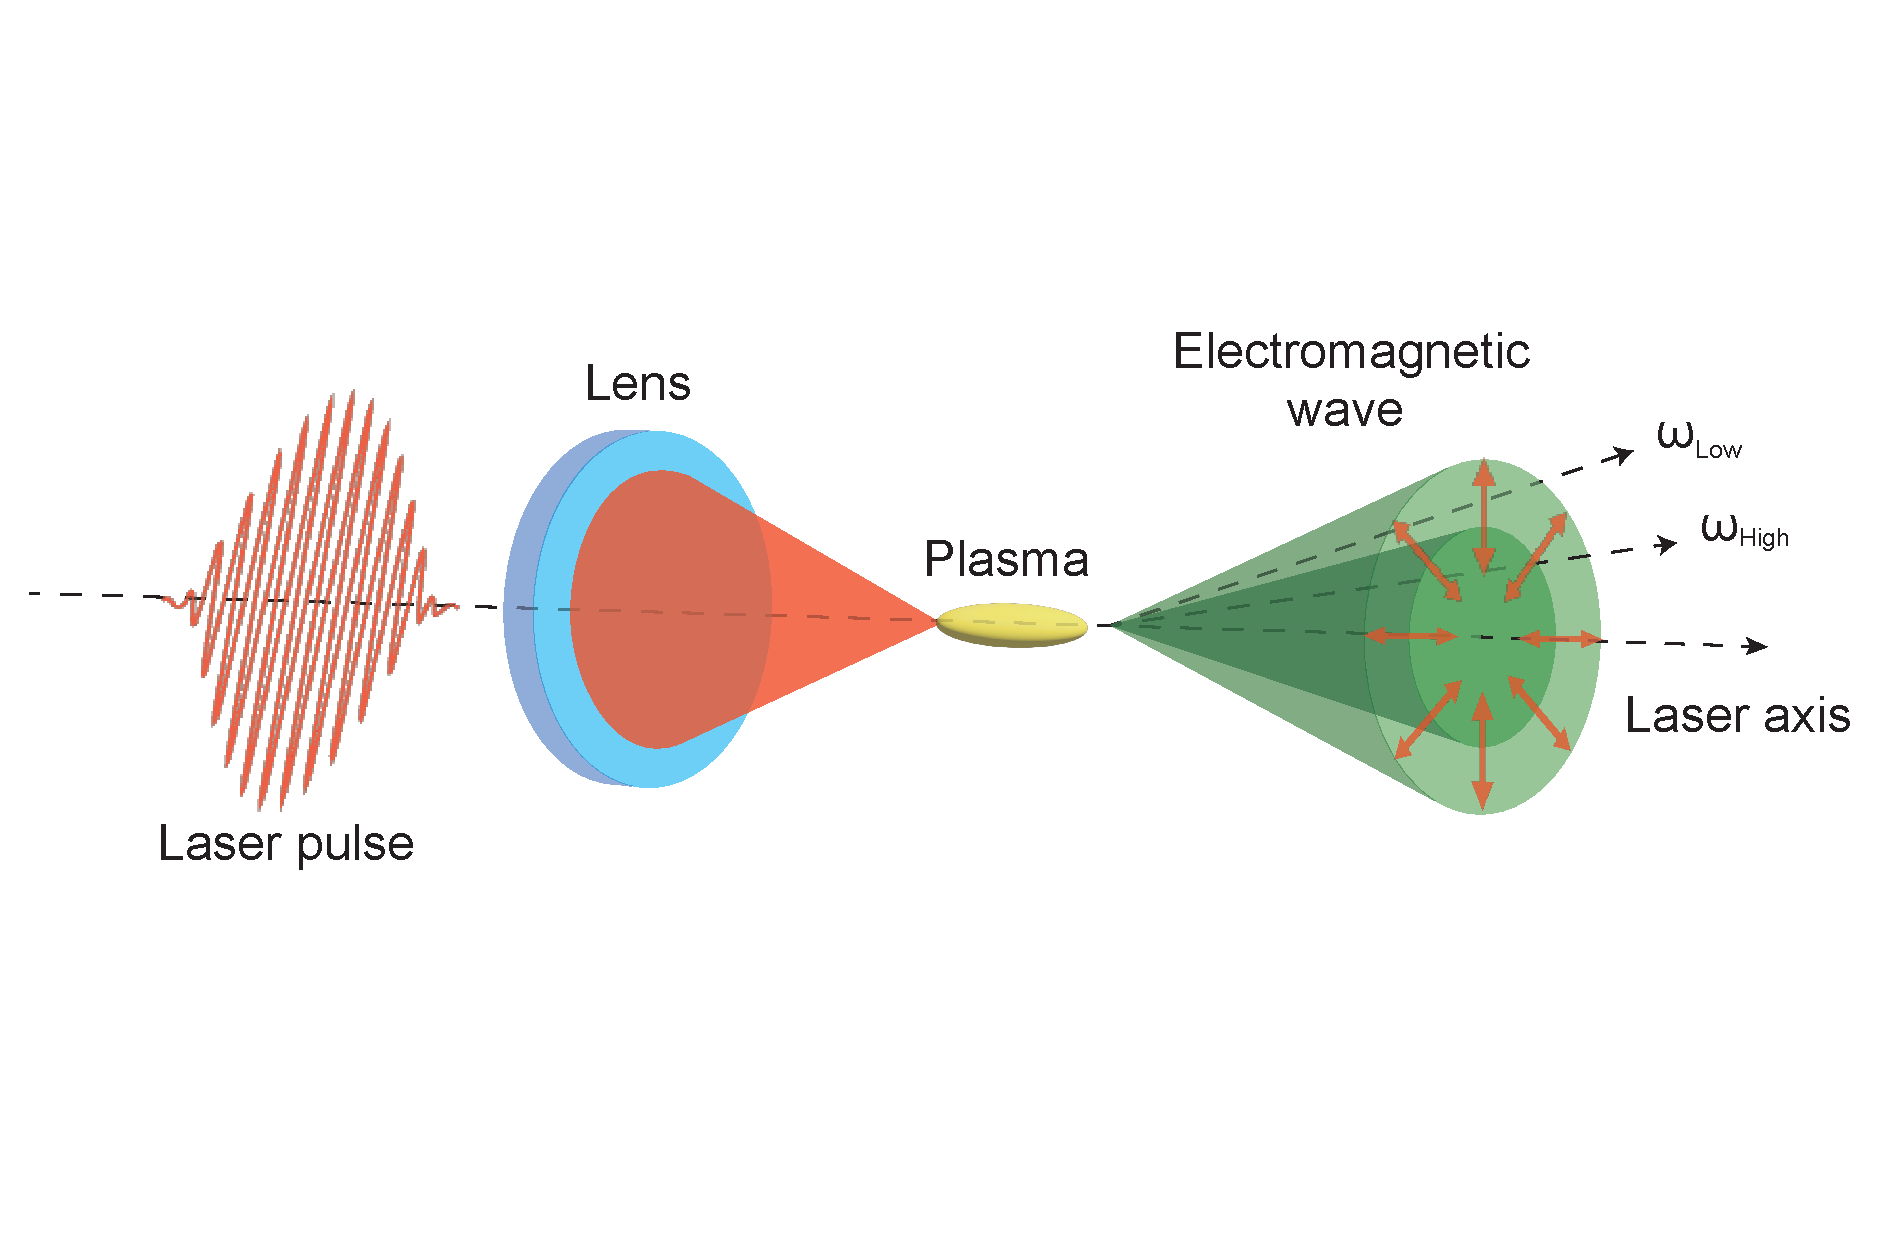
\includegraphics[width=0.46\textwidth]{
        \TWO/Electromagnetic_radiation_by_laser_generated_plasma.pdf
      }
      \caption{レーザー生成プラズマからのテラヘルツ電磁波放射}
      \label{Electromagnetic_radiation_b_laser_generated_plasmay}
    \end{figure}

  \subsection{本講義と研究テーマの関連}
    自身の研究目的は、レーザー生成プラズマからの電磁波放射の原理を解明のため、レーザーによる電離
    やプラズマ生成と密接に関連しています。双極子からの電磁波放射モデルに基づく運動する電荷からの
    電磁波放射の理論はテラヘルツ電磁波放射源からの放射パターンを推定する際に欠かせないと感じてい
    ます。また、プラズマに静電場を印加するため、アンジュレータ光源について学び、研究の理論構築に
    役立てたいと考えています。
